% header.tex -- Beamer preamble for ECON 692 (Spring 2026)
% Compile with XeLaTeX

\documentclass[aspectratio=169, 12pt]{beamer}

% ── Theme ──────────────────────────────────────────────
\usetheme{default}
\usecolortheme{default}
\setbeamertemplate{navigation symbols}{}
\setbeamertemplate{footline}[frame number]

% ── Colors ─────────────────────────────────────────────
\definecolor{usfgreen}{HTML}{00543C}
\definecolor{usfgold}{HTML}{FDBB30}
\definecolor{lightgray}{HTML}{F5F5F5}
\definecolor{codebg}{HTML}{F0F0F0}
\definecolor{darkgray}{HTML}{333333}

\setbeamercolor{title}{fg=usfgreen}
\setbeamercolor{frametitle}{fg=usfgreen}
\setbeamercolor{structure}{fg=usfgreen}
\setbeamercolor{normal text}{fg=darkgray}
\setbeamercolor{itemize item}{fg=usfgreen}
\setbeamercolor{itemize subitem}{fg=usfgreen!80}
\setbeamercolor{itemize subsubitem}{fg=usfgreen!60}
\setbeamercolor{block title}{bg=usfgreen, fg=white}
\setbeamercolor{block body}{bg=lightgray}
\setbeamercolor{footline}{fg=gray}

% ── Fonts ──────────────────────────────────────────────
\usepackage{fontspec}
\setsansfont{Helvetica Neue}[
  BoldFont = {Helvetica Neue Bold},
  ItalicFont = {Helvetica Neue Italic},
]
\setmonofont{Menlo}[Scale=0.85]

% ── Beamer fonts ───────────────────────────────────────
\setbeamerfont{title}{size=\LARGE, series=\bfseries}
\setbeamerfont{subtitle}{size=\large}
\setbeamerfont{frametitle}{size=\Large, series=\bfseries}
\setbeamerfont{framesubtitle}{size=\normalsize}
\setbeamerfont{footline}{size=\tiny}

% ── Frame title formatting ─────────────────────────────
\setbeamertemplate{frametitle}{%
  \vskip6pt%
  \insertframetitle%
  \ifx\insertframesubtitle\empty\else%
    \\[2pt]{\usebeamerfont{framesubtitle}\usebeamercolor[fg]{framesubtitle}\insertframesubtitle}%
  \fi%
  \vskip2pt%
  {\color{usfgreen}\hrule height 1.5pt}%
  \vskip4pt%
}

% ── Title page ─────────────────────────────────────────
\setbeamertemplate{title page}{
  \vfill
  \begin{center}
    {\usebeamerfont{title}\usebeamercolor[fg]{title}\inserttitle}\\[8pt]
    \ifx\insertsubtitle\empty\else
      {\usebeamerfont{subtitle}\usebeamercolor[fg]{subtitle}\insertsubtitle}\\[12pt]
    \fi
    {\color{usfgreen}\rule{0.4\textwidth}{1.5pt}}\\[12pt]
    {\normalsize\insertauthor}\\[4pt]
    {\small\insertinstitute}\\[4pt]
    {\small\insertdate}
  \end{center}
  \vfill
}

% ── Packages ───────────────────────────────────────────
\usepackage{amsmath, amssymb}
\usepackage{graphicx}
\usepackage{tikz}
\usepackage{array}
\usepackage{booktabs}
\usepackage{hyperref}
\hypersetup{colorlinks=true, linkcolor=usfgreen, urlcolor=usfgreen!80}

% ── Code listings ──────────────────────────────────────
\usepackage{listings}
\lstset{
  basicstyle=\ttfamily\small,
  backgroundcolor=\color{codebg},
  frame=single,
  framerule=0pt,
  framexleftmargin=4pt,
  framexrightmargin=4pt,
  framextopmargin=4pt,
  framexbottommargin=4pt,
  breaklines=true,
  showstringspaces=false,
  columns=fullflexible,
  keepspaces=true,
  literate={~}{{\textasciitilde}}1,
}

\lstdefinestyle{terminal}{
  basicstyle=\ttfamily\small\color{darkgray},
  backgroundcolor=\color{codebg},
  language=bash,
}

% ── Itemize bullets ────────────────────────────────────
\setbeamertemplate{itemize item}{\small\raise1pt\hbox{\textbullet}}
\setbeamertemplate{itemize subitem}{\small\raise1pt\hbox{--}}
\setbeamertemplate{itemize subsubitem}{\small\raise1pt\hbox{$\cdot$}}

% ── Useful macros ──────────────────────────────────────
\newcommand{\E}{\mathbb{E}}
\newcommand{\Var}{\mathrm{Var}}
\newcommand{\indep}{\perp\!\!\!\perp}

% ── Section pages ──────────────────────────────────────
\AtBeginSection[]{
  \begin{frame}
    \vfill
    \centering
    {\Large\bfseries\color{usfgreen}\insertsectionhead}
    \vfill
  \end{frame}
}


\title{Research Design \& Causal Inference}
\subtitle{ECON 692 -- Applied Economics Seminar}
\author{Andrew Hobbs}
\institute{University of San Francisco}
\date{February 19, 2026}

\begin{document}

\begin{frame}[plain]
  \titlepage
\end{frame}

% ══════════════════════════════════════════════════════════
%  Agenda & Check-in
% ══════════════════════════════════════════════════════════

\begin{frame}{Today's Agenda}
  \begin{tabular}{@{}r@{\hspace{8pt}}l@{\hspace{16pt}}l@{}}
    \toprule
    \textbf{Time} & \textbf{Duration} & \textbf{Activity} \\
    \midrule
    4:35 & 5 min  & Welcome \& check-in \\
    4:40 & 35 min & Potential outcomes \& DAG theory \\
    5:15 & 25 min & Practical DAG skills \\
    5:40 & 10 min & Break \\
    5:50 & 20 min & DAG software demo \\
    6:10 & 30 min & DAG workshop \\
    6:40 & 10 min & Break \\
    6:50 & 55 min & Empirical strategy drafting \\
    7:45 & 20 min & Share-outs \\
    8:05 & 10 min & Wrap-up \\
    \bottomrule
  \end{tabular}
\end{frame}

\begin{frame}{Check-in}
  \begin{itemize}
    \item How is your data coming together?
    \item Has anyone hit a wall with their data source?
    \item Has anyone started sketching your causal story?
  \end{itemize}
  \vspace{12pt}
  \begin{block}{Reminder}
    Data Report is due \textbf{tomorrow, Friday February 20} at 11:59pm.
  \end{block}
\end{frame}

% ══════════════════════════════════════════════════════════
%  SECTION 1: Potential Outcomes
% ══════════════════════════════════════════════════════════

\section{Potential Outcomes}

\begin{frame}{The Setup: Paid Family Leave}
  \textbf{Research question:} Does access to paid family leave increase female employment?

  \vspace{10pt}

  \begin{itemize}
    \item Unit $i$: a woman in a particular state and year
    \item Treatment: $D_i = 1$ if her state has paid family leave; $0$ otherwise
    \item Outcome: $Y_i = 1$ if employed
  \end{itemize}

  \vspace{10pt}

  \textbf{Potential outcomes:}
  \begin{itemize}
    \item $Y_i(1)$: her employment \textit{if} her state \textbf{has} PFL
    \item $Y_i(0)$: her employment \textit{if} her state does \textbf{not} have PFL
  \end{itemize}

  \vspace{8pt}

  We observe: $Y_i = D_i \cdot Y_i(1) + (1-D_i) \cdot Y_i(0)$ \quad -- only \textbf{one} potential outcome per unit.
\end{frame}

\begin{frame}{The Fundamental Problem}
  \textbf{Individual treatment effect:}\quad $\tau_i = Y_i(1) - Y_i(0)$

  \vspace{6pt}

  This is \textbf{never observed} -- we cannot put the same woman simultaneously in a PFL state and a non-PFL state.

  \vspace{10pt}

  \textbf{So we estimate averages:}

  \vspace{6pt}

  \begin{tabular}{@{}ll@{}}
    $\text{ATE} = \E[Y_i(1) - Y_i(0)]$            & Effect averaged over \textit{everyone} \\[6pt]
    $\text{ATT} = \E[Y_i(1) - Y_i(0) \mid D_i=1]$ & Effect averaged over the \textit{treated} \\
  \end{tabular}

  \vspace{10pt}

  For policy evaluation, we usually want the \textbf{ATT}.

  \vspace{4pt}

  \textit{``Did PFL raise employment for women in states that adopted it?''}
\end{frame}

\begin{frame}{Selection Bias}
  \small
  The naive comparison mixes up the treatment effect with pre-existing differences:

  \vspace{4pt}

  \[
    \E[Y_i \mid D_i=1] - \E[Y_i \mid D_i=0]
    \;=\; \E[Y_i(1) \mid D_i=1] - \E[Y_i(0) \mid D_i=0]
  \]

  \vspace{2pt}

  Add and subtract $\E[Y_i(0) \mid D_i=1]$:

  \[
    =\;
    \underbrace{\E[Y_i(1) - Y_i(0) \mid D_i=1]}_{\text{ATT (what we want)}}
    \;+\;
    \underbrace{\E[Y_i(0) \mid D_i=1] - \E[Y_i(0) \mid D_i=0]}_{\text{Selection bias}}
  \]

  \vspace{6pt}

  \normalsize
  \textbf{Selection bias for PFL:} states that adopt PFL may have had higher female employment \textit{even without} the policy -- liberal, urban states pass PFL \textit{and} have stronger female labor markets.

  \vspace{4pt}

  The naive comparison cannot tell us whether high employment in PFL states reflects $\tau$ or pre-existing advantages.
\end{frame}

\begin{frame}{Where Does Bias Come From?}
  Potential outcomes \textbf{define} the target and \textbf{name} the problem.

  \vspace{8pt}

  But they don't tell us \textit{where} the bias comes from or \textit{what to condition on} to remove it.

  \vspace{10pt}

  \begin{tabular}{@{}ll@{}}
    \toprule
    \textbf{Potential outcomes} & \textbf{DAGs} \\
    \midrule
    Define the estimand (ATE, ATT) & Map the data-generating process \\
    Name the problem (selection bias) & Show \textit{where} bias enters \\
    \textit{What} to estimate & \textit{How} to identify it \\
    \bottomrule
  \end{tabular}

  \vspace{12pt}

  \textit{Use potential outcomes to define your target. Use DAGs to design your identification strategy.}
\end{frame}

% ══════════════════════════════════════════════════════════
%  SECTION 2: DAGs
% ══════════════════════════════════════════════════════════

\section{Directed Acyclic Graphs}

\begin{frame}{DAG Building Blocks}
  A \textbf{Directed Acyclic Graph} is a map of your causal assumptions.

  \vspace{10pt}

  \begin{itemize}
    \item \textbf{Nodes}: variables (observed or unobserved)
    \item \textbf{Directed edges}: $X \to Y$ means ``$X$ has a direct causal effect on $Y$,
          holding all other variables fixed''
    \item \textbf{Acyclic}: no feedback loops
  \end{itemize}

  \vspace{10pt}

  \begin{block}{Key insight}
    Every missing arrow is also an assumption: ``these two things are not directly connected.''
    A DAG encodes your \textbf{substantive theory}, not just your statistical model.
  \end{block}
\end{frame}

\begin{frame}{Three Fundamental Structures}
  \small
  \begin{columns}[T]
    \begin{column}{0.32\textwidth}
      \centering
      \textbf{Fork (Confounder)}\\[8pt]
      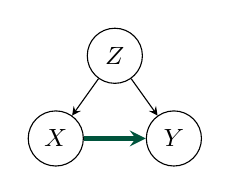
\begin{tikzpicture}[>=stealth, scale=0.75]
        \node[draw, circle, minimum size=0.7cm, font=\small] (Z) at (0, 1.4) {$Z$};
        \node[draw, circle, minimum size=0.7cm, font=\small] (X) at (-1, 0) {$X$};
        \node[draw, circle, minimum size=0.7cm, font=\small] (Y) at (1, 0) {$Y$};
        \draw[->] (Z) -- (X);
        \draw[->] (Z) -- (Y);
        \draw[->, usfgreen, line width=1.5pt] (X) -- (Y);
      \end{tikzpicture}\\[6pt]
      $Z$ opens a backdoor path\\[6pt]
      \textbf{\textcolor{usfgreen}{Block it:}}\\condition on $Z$
    \end{column}
    \begin{column}{0.32\textwidth}
      \centering
      \textbf{Chain (Mediator)}\\[8pt]
      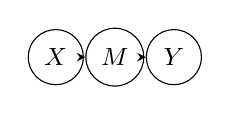
\begin{tikzpicture}[>=stealth, scale=0.75]
        \node[draw, circle, minimum size=0.7cm, font=\small] (X) at (-1, 0.7) {$X$};
        \node[draw, circle, minimum size=0.7cm, font=\small] (M) at (0, 0.7) {$M$};
        \node[draw, circle, minimum size=0.7cm, font=\small] (Y) at (1, 0.7) {$Y$};
        \draw[->] (X) -- (M);
        \draw[->] (M) -- (Y);
      \end{tikzpicture}\\[6pt]
      $X$ affects $Y$ through $M$\\[6pt]
      \textbf{\textcolor{red}{Caution:}}\\conditioning on $M$\\blocks this path
    \end{column}
    \begin{column}{0.32\textwidth}
      \centering
      \textbf{Collider}\\[8pt]
      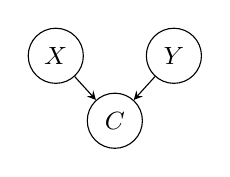
\begin{tikzpicture}[>=stealth, scale=0.75]
        \node[draw, circle, minimum size=0.7cm, font=\small] (X) at (-1, 0.8) {$X$};
        \node[draw, circle, minimum size=0.7cm, font=\small] (C) at (0, -0.3) {$C$};
        \node[draw, circle, minimum size=0.7cm, font=\small] (Y) at (1, 0.8) {$Y$};
        \draw[->] (X) -- (C);
        \draw[->] (Y) -- (C);
      \end{tikzpicture}\\[6pt]
      Both $X$ and $Y$ cause $C$\\[6pt]
      \textbf{\textcolor{red}{Danger:}}\\conditioning on $C$\\\textit{opens} a spurious path
    \end{column}
  \end{columns}
\end{frame}

\begin{frame}{The Fork: Confounders}
  \begin{columns}[T]
    \begin{column}{0.47\textwidth}
      \centering
      \vspace{6pt}
      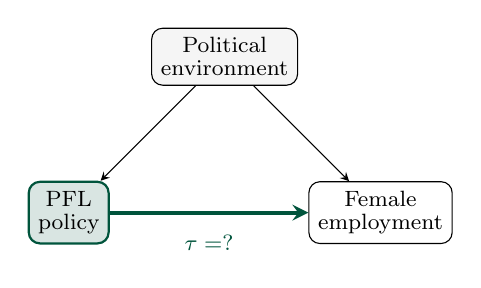
\begin{tikzpicture}[>=stealth, scale=0.9]
        \node[draw, rounded corners, font=\footnotesize, fill=lightgray]
          (POL) at (2.2, 2.2) {\shortstack{Political\\environment}};
        \node[draw, rounded corners, font=\footnotesize, fill=usfgreen!15, draw=usfgreen, thick]
          (PFL) at (0, 0) {\shortstack{PFL\\policy}};
        \node[draw, rounded corners, font=\footnotesize]
          (EMP) at (4.4, 0) {\shortstack{Female\\employment}};
        \draw[->] (POL) -- (PFL);
        \draw[->] (POL) -- (EMP);
        \draw[->, usfgreen, line width=1.5pt] (PFL) -- (EMP)
          node[midway, below, yshift=-4pt, font=\footnotesize, usfgreen] {$\tau = ?$};
      \end{tikzpicture}
    \end{column}
    \begin{column}{0.50\textwidth}
      \textbf{Backdoor path:}\; PFL $\leftarrow$ POL $\rightarrow$ EMP

      \vspace{8pt}

      \begin{itemize}
        \item Liberal states adopt PFL earlier
        \item Liberal states also have stronger female labor markets for \textit{other} reasons
        \item Naive comparison cannot separate $\tau$ from the POL effect
      \end{itemize}

      \vspace{8pt}

      \textbf{\textcolor{usfgreen}{Block the backdoor:}} condition on political environment to isolate $\tau$

      \textit{In practice:} state fixed effects, vote-share controls, ideology index
    \end{column}
  \end{columns}
\end{frame}

\begin{frame}{The Chain: Mediators}
  \small
  \begin{columns}[T]
    \begin{column}{0.48\textwidth}
      \centering
      \vspace{4pt}
      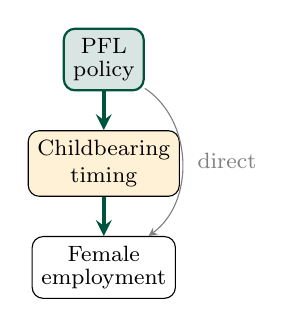
\begin{tikzpicture}[>=stealth, scale=0.88]
        \node[draw, rounded corners, font=\footnotesize, fill=usfgreen!15, draw=usfgreen, thick]
          (PFL) at (0, 3.0) {\shortstack{PFL\\policy}};
        \node[draw, rounded corners, font=\footnotesize, fill=usfgold!20]
          (CHILD) at (0, 1.5) {\shortstack{Childbearing\\timing}};
        \node[draw, rounded corners, font=\footnotesize]
          (EMP) at (0, 0) {\shortstack{Female\\employment}};
        % Chain path (mediator)
        \draw[->, usfgreen, line width=1.5pt] (PFL) -- (CHILD);
        \draw[->, usfgreen, line width=1.5pt] (CHILD) -- (EMP);
        % Direct path (solid gray -- distinct from chain path)
        \draw[->, gray]
          (PFL) to[bend left=55]
          node[right, xshift=2pt, font=\footnotesize, gray] {direct} (EMP);
      \end{tikzpicture}
    \end{column}
    \begin{column}{0.49\textwidth}
      \begin{itemize}
        \item PFL enables women to have children \textit{and} remain employed -- a core mechanism
        \item Both paths are genuine effects of PFL; controlling for childbearing blocks one and \textbf{underestimates} the total effect
      \end{itemize}

      \vspace{4pt}

      \textbf{Rule:} do \textbf{not} condition on mediators unless you want the \textit{direct} effect only, net of the mechanism.
    \end{column}
  \end{columns}
\end{frame}

\begin{frame}{The Collider: A Subtle Danger}
  \small
  \begin{columns}[T]
    \begin{column}{0.48\textwidth}
      \centering
      \vspace{6pt}
      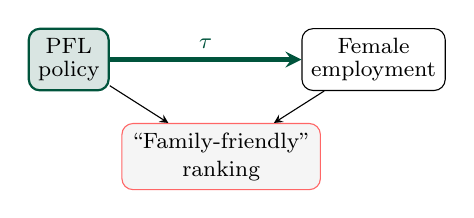
\begin{tikzpicture}[>=stealth, scale=0.88]
        \node[draw, rounded corners, font=\footnotesize, fill=usfgreen!15, draw=usfgreen, thick]
          (PFL) at (0, 1.4) {\shortstack{PFL\\policy}};
        \node[draw, rounded corners, font=\footnotesize]
          (EMP) at (4.4, 1.4) {\shortstack{Female\\employment}};
        \node[draw=red!60, rounded corners, font=\footnotesize, fill=lightgray]
          (RANK) at (2.2, 0) {\shortstack{``Family-friendly''\\ranking}};
        \draw[->] (PFL) -- (RANK);
        \draw[->] (EMP) -- (RANK);
        \draw[->, usfgreen, line width=1.5pt] (PFL) -- (EMP)
          node[midway, above, font=\footnotesize, usfgreen] {$\tau$};
      \end{tikzpicture}
    \end{column}
    \begin{column}{0.49\textwidth}
      \footnotesize
      Both PFL adoption and high female employment feed into ``family-friendly'' rankings.

      \vspace{4pt}

      \begin{itemize}
        \item Collider paths are \textbf{closed by default} -- no bias
        \item Restricting your sample to highly-ranked states conditions on the collider -- opening a spurious path
      \end{itemize}

      \vspace{4pt}

      \textbf{\textcolor{red}{Rule:}} do not condition on variables caused by both $X$ and $Y$ -- e.g., selecting on outcomes or post-treatment variables.
    \end{column}
  \end{columns}
\end{frame}

\begin{frame}{The PFL DAG}
  \begin{columns}[T]
    \begin{column}{0.57\textwidth}
      \centering
      \vspace{4pt}
      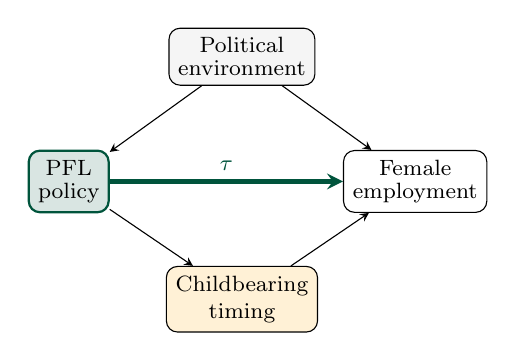
\begin{tikzpicture}[>=stealth, scale=0.88]
        \node[draw, rounded corners, font=\footnotesize, fill=lightgray]
          (POL) at (2.5, 3) {\shortstack{Political\\environment}};
        \node[draw, rounded corners, font=\footnotesize, fill=usfgreen!15, draw=usfgreen, thick]
          (PFL) at (0, 1.2) {\shortstack{PFL\\policy}};
        \node[draw, rounded corners, font=\footnotesize]
          (EMP) at (5, 1.2) {\shortstack{Female\\employment}};
        \node[draw, rounded corners, font=\footnotesize, fill=usfgold!20]
          (CHILD) at (2.5, -0.5) {\shortstack{Childbearing\\timing}};
        % Treatment effect
        \draw[->, usfgreen, line width=1.5pt] (PFL) -- (EMP)
          node[midway, above, font=\footnotesize, usfgreen] {$\tau$};
        % Confounders
        \draw[->] (POL) -- (PFL);
        \draw[->] (POL) -- (EMP);
        % Mediator
        \draw[->] (PFL) -- (CHILD);
        \draw[->] (CHILD) -- (EMP);
      \end{tikzpicture}
    \end{column}
    \begin{column}{0.40\textwidth}
      \small
      \textbf{Backdoor path (bias):}
      \begin{itemize}
        \item PFL $\leftarrow$ POL $\rightarrow$ EMP
      \end{itemize}

      \vspace{8pt}

      \textbf{Mediator (don't control):}
      \begin{itemize}
        \item PFL $\to$ CHILD $\to$ EMP
      \end{itemize}

      \vspace{8pt}

      \textbf{Minimum adjustment set:}
      \begin{itemize}
        \item \textbf{\{Political environment\}}
      \end{itemize}

      \vspace{8pt}

      Controlling for POL closes the backdoor path without blocking the treatment effect.
    \end{column}
  \end{columns}
\end{frame}

\begin{frame}{The Backdoor Criterion}
  \begin{block}{Backdoor Criterion (Pearl, 2009)}
    A set of variables $\mathbf{Z}$ identifies the causal effect of $X$ on $Y$ if:
    \begin{enumerate}
      \item No variable in $\mathbf{Z}$ is a \textbf{descendant} of $X$ (no mediators or outcomes)
      \item $\mathbf{Z}$ \textbf{blocks every path} between $X$ and $Y$ that begins with an arrow \textit{into} $X$
    \end{enumerate}
  \end{block}

  \vspace{6pt}

  \textbf{Applied to PFL:}
  \begin{itemize}
    \item Backdoor path: PFL $\leftarrow$ POL $\rightarrow$ EMP
    \item Adjustment set $\{$POL$\}$: blocks the path; POL is not a descendant of PFL \checkmark
    \item \textbf{Do not} include CHILD -- descendant of PFL (violates condition 1)
  \end{itemize}

  \vspace{4pt}

  \textit{Practical shortcut:} \texttt{dagitty.net} finds the adjustment set automatically.
\end{frame}

\begin{frame}{DAGs and Parallel Trends}
  \small
  \textbf{Parallel trends requires:} absent PFL, treated and control states would have followed the same employment trajectory.

  \vspace{4pt}

  \textbf{When does this fail?} When a confounder $Z$ satisfies all three:
  \begin{enumerate}
    \item $Z \to$ PFL adoption \textit{timing}
    \item $Z \to$ EMP over \textit{time} (affects trends, not just levels)
    \item $Z$ is not controlled for
  \end{enumerate}

  \vspace{4pt}

  In the PFL DAG: political environment drove both adoption timing and employment growth -- early adopters will diverge from controls before the policy, which a pre-trends test detects.

  \vspace{6pt}

  \textbf{Practical rule:} check your DAG before running your event study. Every time-varying confounder is a candidate for a parallel trends violation -- and a robustness check to add.
\end{frame}

% ══════════════════════════════════════════════════════════
%  SECTION 3: DAG Software
% ══════════════════════════════════════════════════════════

\section{DAG Software}

\begin{frame}{dagitty.net}
  \textbf{Free, browser-based -- no installation required.}

  \vspace{8pt}

  \begin{columns}[T]
    \begin{column}{0.54\textwidth}
      \textbf{What it does:}
      \begin{itemize}
        \item Draw nodes and edges with point-and-click
        \item Specify treatment, outcome, observed variables
        \item Automatically finds: adjustment sets, testable implications, all open paths
      \end{itemize}
    \end{column}
    \begin{column}{0.43\textwidth}
      \textbf{Quick start:}
      \begin{enumerate}
        \item Go to \texttt{dagitty.net}
        \item \textit{Model} $\to$ \textit{New Model}
        \item Click to add nodes; drag to connect
        \item Right-click a node to mark it as treatment or outcome
        \item Read the \textbf{Adjustment} panel
      \end{enumerate}
    \end{column}
  \end{columns}

  \vspace{8pt}

  Use this during the workshop: enter your project DAG and let dagitty find your adjustment set.
\end{frame}

\begin{frame}[fragile]{ggdag in R}
  For publication-quality figures in your paper or final presentation.

  \vspace{6pt}

\begin{lstlisting}[style=terminal]
library(ggdag)

pfl_dag <- dagify(EMP ~ PFL + POL + CHILD,
                  PFL ~ POL, CHILD ~ PFL,
                  exposure = "PFL", outcome = "EMP")

ggdag(pfl_dag, layout = "sugiyama") + theme_dag()
ggdag_adjustment_set(pfl_dag)
\end{lstlisting}

  \vspace{4pt}

  \texttt{install.packages("ggdag")} -- also installs \texttt{dagitty} as a dependency.
\end{frame}

% ══════════════════════════════════════════════════════════
%  SECTION 4: DAG Workshop
% ══════════════════════════════════════════════════════════

\section{DAG Workshop}

\begin{frame}{Draw Your DAG}
  \textbf{Step 1 -- Individual (15 minutes)}

  For your own research project, draw a DAG that includes:
  \begin{itemize}
    \item Your \textbf{treatment} and \textbf{outcome}, clearly labeled
    \item At least \textbf{two confounders} (forks -- things that affect both treatment and outcome)
    \item At least \textbf{one mediator}, if applicable (a mechanism through which treatment operates)
    \item Mark what you plan to \textbf{condition on} -- and why
  \end{itemize}

  Use paper, a whiteboard, or \texttt{dagitty.net}.

  \vspace{4pt}

  \textbf{Step 2 -- Groups of 3 (15 minutes)}

  Share your DAG. For each person, the group asks:
  \begin{itemize}
    \item What is the main backdoor path?
    \item Does the adjustment set satisfy the backdoor criterion?
    \item Is anything being controlled that shouldn't be (a mediator or collider)?
  \end{itemize}
\end{frame}

% ══════════════════════════════════════════════════════════
%  SECTION 5: Empirical Strategy Drafting
% ══════════════════════════════════════════════════════════

\section{Empirical Strategy Drafting}

\begin{frame}{Drafting Sprint}
  \textbf{55 minutes.} This starts your \textbf{Empirical Strategy Draft} -- due \textbf{March 6}, a separate submission from the Data Report.

  \vspace{6pt}

  Write \textbf{2--3 paragraphs} covering:

  \begin{enumerate}
    \item \textbf{Identification strategy} -- what variation are you exploiting? Why is it plausibly exogenous? Name the method and the specific source of variation.

    \item \textbf{Causal diagram} -- what does your DAG imply about what you need to control for? Be explicit: which confounders will you include and why? Which variables will you \textit{not} control for, and why not?

    \item \textbf{Main threat and response} -- what is the single biggest threat to your identification? How will you address or test it (robustness check, placebo test, pre-trends plot)?
  \end{enumerate}

  \vspace{4pt}

  \textit{Goal: a rough draft to build on over the next two weeks. I'll be circulating.}
\end{frame}

\begin{frame}{Share-outs}
  \textbf{3--4 students, 5 minutes each.}

  \vspace{12pt}

  Cover:
  \begin{enumerate}
    \item \textbf{Research question} -- one sentence
    \item \textbf{Key finding from your DAG} -- what was the most important backdoor path you identified? How are you addressing it?
    \item \textbf{Main identification threat} -- and your plan for testing or addressing it
  \end{enumerate}

  \vspace{12pt}

  Listeners: one piece of feedback each.
\end{frame}

\begin{frame}{Wrap-Up \& Next Week}
  \textbf{Due this week:}
  \begin{itemize}
    \item \textbf{Data Report -- due tomorrow, Friday February 20}
    \item Weekly progress report (Friday)
  \end{itemize}

  \vspace{10pt}

  \textbf{Next week (Week 5):}
  \begin{itemize}
    \item Data cleaning and merging for reproducibility
    \item Hands-on implementation with your own data
  \end{itemize}

  \vspace{10pt}

  \textbf{Before next class:}
  \begin{itemize}
    \item Submit your Data Report
    \item Make sure your data loads cleanly in R or Python
    \item Push your current code to GitHub
    \item Revisit your DAG -- refine it based on today's feedback
  \end{itemize}
\end{frame}

\end{document}
